
% variational-autoencoder.tex

\documentclass[dvipdfmx,notheorems,t]{beamer}

\usepackage{docmute}

% settings.tex

\AtBeginDvi{\special{pdf:tounicode 90ms-RKSJ-UCS2}}

\AtBeginSection[]{\frame[t]{\frametitle{目次}
	\tableofcontents[currentsection,hideallsubsections]}}

\AtBeginSubsection[]{\frame[t]{\frametitle{目次}
	\tableofcontents[currentsection,currentsubsection,subsectionstyle=show/shaded/hide]}}

\usefonttheme{professionalfonts}
\usetheme{Madrid}

\setbeamercovered{transparent=30} 
% \setbeamertemplate{navigation symbols}{}
\setbeamertemplate{frametitle}[default][left]
\setbeamertemplate{frametitle continuation}{}
\setbeamertemplate{enumerate items}[square]
\setbeamertemplate{caption}[numbered]

\let\oldframe\frame
\renewcommand\frame[1][allowdisplaybreaks,allowframebreaks,t]{\oldframe[#1]}

\usepackage{bxdpx-beamer}
\usepackage{pxjahyper}
\usepackage{minijs}

\usepackage{amsmath}
\usepackage{amssymb}
\usepackage{amsthm}
\usepackage{bm}

\DeclareMathOperator*{\argmax}{arg\,max}
\DeclareMathOperator*{\argmin}{arg\,min}
\DeclareMathOperator{\Tr}{Tr}
\DeclareMathOperator{\KL}{KL}
\DeclareMathOperator{\diag}{diag}

\usepackage[T1]{fontenc}
\usepackage[utf8]{inputenc}

\setbeamertemplate{theorems}[numbered]
\theoremstyle{definition}
\newtheorem{theorem}{定理}
\newtheorem{definition}{定義}
\newtheorem{proposition}{命題}
\newtheorem{lemma}{補題}
\newtheorem{corollary}{系}
\newtheorem{conjecture}{予想}
\newtheorem*{remark}{Remark}
\renewcommand{\proofname}{}

\renewcommand{\figurename}{図}
\renewcommand{\tablename}{表}

\renewcommand{\kanjifamilydefault}{\gtdefault}


\begin{document}

\section{変分自己符号化器}

\subsection{生成モデル}

\begin{frame}{生成モデル}

\begin{itemize}
	\item 生成モデルの目的
	\begin{itemize}
		\item データ$\bm{x}$に関する分布$p(\bm{x})$を推定する
	\end{itemize} \
	
	\item データ生成過程
	\begin{itemize}
		\item データ$\bm{x}$は一般に高次元である
		\item 但し、実際にデータが分布しているのは、ごく限られた一部の低次元の領域であると考えられる (\alert{多様体仮説})
		\item データ$\bm{x}$自体は高次元だが、本質的には低次元の情報しか持たないと考えられる
		\newline
		
		\item データ$\bm{x}$を、より低次元なベクトル$\bm{z}$を使って、表現することを考える
		\item データに関する分布$p(\bm{x})$を、潜在変数$\bm{z}$に関する分布と、うまく組み合わせて記述する
		\item \alert{潜在変数からデータが生成されるまでの過程}を組み込んで、$p(\bm{x})$を記述する
	\end{itemize}
\end{itemize}

\end{frame}

\subsection{変分自己符号化器(VAE)の概要}

\begin{frame}{変分自己符号化器(VAE)の概要}

\begin{itemize}
	\item 深層学習における生成モデル
	\begin{itemize}
		\item 主に以下の2つの手法が存在する
		\newline
		
		\item 敵対的生成ネットワーク (Generative Adversarial Networks, GAN)
		\item \alert{変分自己符号化器} (Variational Auto Encoders, \alert{VAE})
		\newline
		
		\item ここでは変分自己符号化器(VAE)について扱う
		\newline
		
		\item VAEを、異常検知(不良品の検出など)に使った例がある
	\end{itemize}
\end{itemize}

\end{frame}

\begin{frame}{変分自己符号化器(VAE)の概要}

\begin{itemize}
	\item VAEにおけるグラフィカルモデル
	\begin{itemize}
		\item 図\ref{fig:vae-graphical-model}のような、潜在変数を含んだグラフィカルモデルを考える
		\newline
		
		\item データ$\bm{x}$について、ある一つの潜在変数$\bm{z}$が対応しているとする
		\item 各データ$\bm{x}$は、分布$p(\bm{x})$から独立にサンプルされるとする
		\item 従って、データ$\left\{ \bm{x}_1, \ldots, \bm{x}_N \right\}$は\alert{独立同分布標本}とする
		\newline
		
		\item $\theta$は、\color{red}潜在変数$\bm{z}$からデータ$\bm{x}$\normalcolor を取得する際に使用されるパラメータ
		\item $\phi$は、\color{red}データ$\bm{x}$から潜在変数$\bm{z}$\normalcolor を生成する際に使用されるパラメータ
		\item $N$は、データ数である
	\end{itemize}
\end{itemize}

\end{frame}

\begin{frame}{変分自己符号化器(VAE)の概要}

\begin{itemize}
	\item データ$\bm{x}$の生成過程
	\begin{itemize}
		\item データ$\bm{x}$の生成過程は、次のように考える
		\newline
		\item 分布\color{red}$p(\bm{z} | \theta)$\normalcolor から、潜在変数$\bm{z}_i$がサンプルされる
		\item 分布\color{red}$p(\bm{x} | \bm{z}_i, \theta)$\normalcolor から、データ$\bm{x}_i$がサンプルされる
		\newline
		
		\item これより、データ$\bm{x}$の分布を次のように表現できる
		\begin{equation}
			p(\bm{x} | \theta) = \int p(\bm{x} | \bm{z}, \theta) p(\bm{z} | \theta) d\bm{z}
		\end{equation}
	\end{itemize} \
	
	\item 潜在変数$\bm{z}$をデータ$\bm{x}$から取得する過程
	\begin{itemize}
		\item 潜在変数$\bm{z}_i$をデータ$\bm{x}_i$から得る過程は、次のように考える
		\newline
		\item 分布\color{red}$q(\bm{z} | \bm{x}_i, \phi)$\normalcolor から、潜在変数$\bm{z}_i$がサンプルされる
	\end{itemize}
\end{itemize}

\end{frame}

\begin{frame}{変分自己符号化器(VAE)の概要}

\begin{figure}
	\centering
	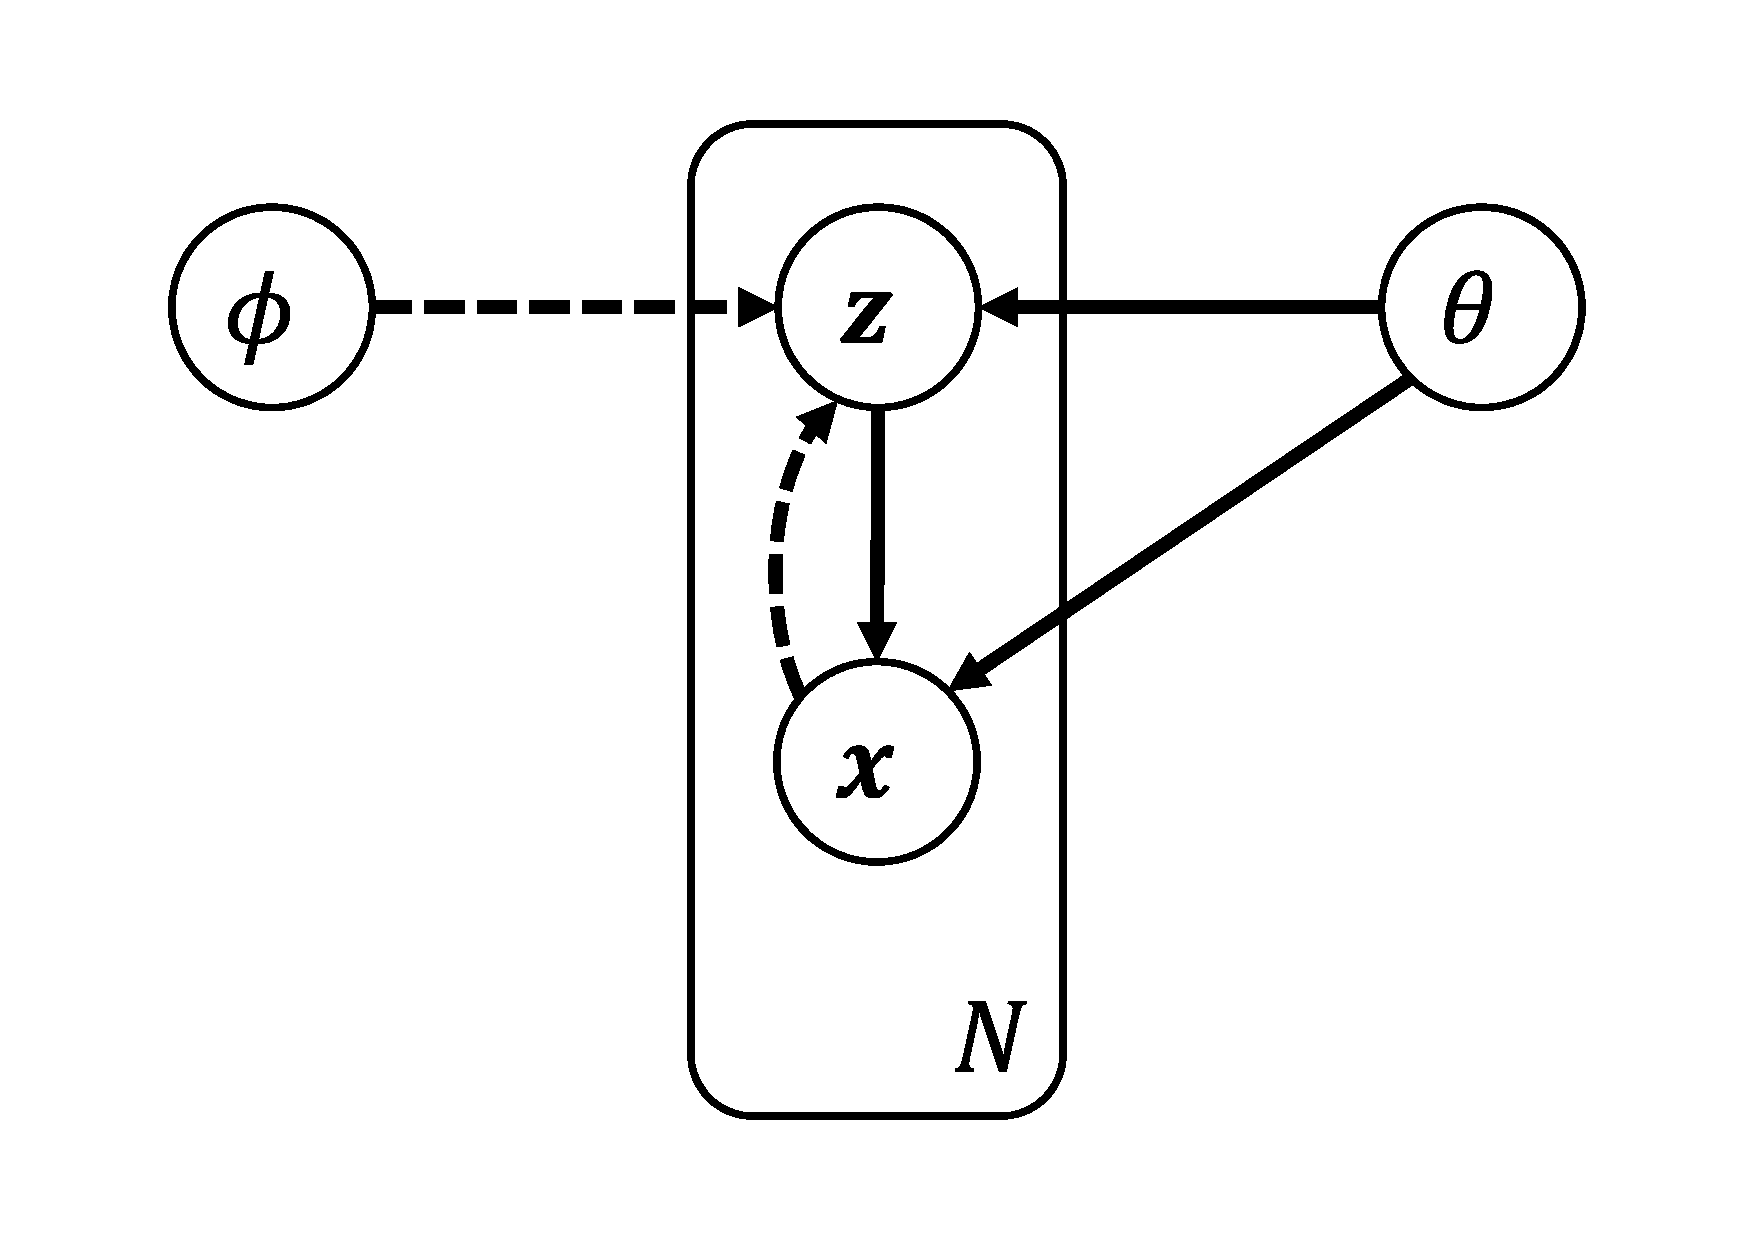
\includegraphics[keepaspectratio,scale=0.2]{vae-graphical-model.pdf}
	\caption{変分自己符号化器(VAE)におけるグラフィカルモデル}
	\label{fig:vae-graphical-model}
\end{figure}

\end{frame}

\begin{frame}{変分自己符号化器(VAE)の概要}

\begin{itemize}
	\item 確率分布のニューラルネットワークによる表現
	\begin{itemize}
		\item 潜在変数を含む確率モデルについて、パラメータの最尤解を求めるために、EMアルゴリズムを導出した
		\item EMアルゴリズムでは、潜在変数に関する事後分布$p(\bm{z} | \bm{x}, \theta)$を計算する必要があった
		\item この事後分布$p(\bm{z} | \bm{x}, \theta)$の計算が困難であるとき、$p(\bm{z} | \bm{x})$を別の分布$q(\bm{z} | \bm{x}, \phi)$で近似し、変分推論によって$q(\bm{z} | \phi)$の最適解を求めた
		\newline
		\item VAEは変分推論の変種であり、近似事後分布$q(\bm{z} | \bm{x}, \phi)$と、$p(\bm{x} | \bm{z})$の2つを\alert{ニューラルネットワーク}で表現する
		\newline
		\item データ$\bm{x}$を潜在変数$\bm{z}$に対応付けるニューラルネットワークを、\alert{Encoder}という
		\item 潜在変数$\bm{z}$からデータ$\bm{x}$を復元するニューラルネットワークを、\alert{Decoder}という
		\item 分布$q(\bm{z} | \bm{x}, \phi)$は\alert{Encoder}、分布$p(\bm{x} | \bm{z}, \theta)$は\alert{Encoder}に相当する
	\end{itemize}
\end{itemize}

\end{frame}

\subsection{変分自己符号化器(VAE)の理論}

\begin{frame}{変分自己符号化器(VAE)の理論}

\begin{itemize}
	\item 変分自己符号化器(VAE)の理論
	\begin{itemize}
		\item 変分下界$\mathcal{L}(q)$は次のようであった
		\begin{eqnarray}
			\mathcal{L}(q) &=& \int q(\bm{z} | \bm{x}) \ln \frac{p(\bm{x}, \bm{z})}{q(\bm{z} | \bm{x})} d\bm{z} \\
			&=& \int q(\bm{z} | \bm{x}) \ln \frac{p(\bm{x} | \bm{z}) p(\bm{z})}{q(\bm{z} | \bm{x})} d\bm{z} \\
			&=& \int q(\bm{z} | \bm{x}) \ln p(\bm{x} | \bm{z}) d\bm{z} + \int q(\bm{z} | \bm{x}) \ln \frac{p(\bm{z})}{q(\bm{z} | \bm{x})} d\bm{z} \\
			&=& \int q(\bm{z} | \bm{x}) \ln p(\bm{x} | \bm{z}) d\bm{z} - \KL(q(\bm{z} | \bm{x}) || p(\bm{z})) \\
			&=& \mathbb{E}_{\bm{z} \sim q(\bm{z} | \bm{x})} \left[ \ln p(\bm{x} | \bm{z}) \right] - \KL(q(\bm{z} | \bm{x}) || p(\bm{z}))
		\end{eqnarray}
		
		\item ここでは、単一のデータ$\bm{x}$と、それに対応する潜在変数$\bm{z}$を考えている
		\item また、パラメータ$\theta, \phi$は省略している
		\newline
		
		\item \alert{第1項}$\mathbb{E}_{\bm{z} \sim q(\bm{z} | \bm{x})} \left[ \ln p(\bm{x} | \bm{z}) \right]$を\alert{大きく}、また\alert{第2項}$\KL(q(\bm{z} | \bm{x}) || p(\bm{z}))$を\alert{小さく}することで、変分下界$\mathcal{L}(q)$を大きくできる
		\newline
		\item VAEでは、変分下界$\mathcal{L}(q)$を最大化するパラメータ$\theta, \phi$を求めるために、ニューラルネットを使用する (変分推論にニューラルネットをねじ込んだもの)
		\newline
		
		\item KLダイバージェンスの項は、後ほど求めることにする(解析的に求められる)
		\item 第1項は、分布$q(\bm{z} | \bm{x})$に関する期待値であり、VAEでは\alert{サンプリングで近似}する
		\begin{equation}
			\mathbb{E}_{\bm{z} \sim q(\bm{z} | \bm{x})} \left[ \ln p(\bm{x} | \bm{z}) \right] \simeq \frac{1}{L} \sum_{l = 1}^L \ln p(\bm{x}_i | \bm{z}_{i, l})
		\end{equation}
		
		\item これより、変分下界$\mathcal{L}(q)$は以下のように書ける
		\begin{equation}
			\mathcal{L}(q) \simeq -\KL(q(\bm{z} | \bm{x}) || p(\bm{z})) + \frac{1}{L} \sum_{i = 1}^L \ln p(\bm{x}_i | \bm{z}_{i, l})
		\end{equation}
		
		\item パラメータ$\theta, \phi$を含めれば、次のように書ける
		\begin{equation}
			\mathcal{L}(q) \simeq -\KL(q(\bm{z} | \bm{x}, \phi) || p(\bm{z} | \theta)) + \frac{1}{L} \sum_{i = 1}^L \ln p(\bm{x}_i | \bm{z}_{i, l}, \theta)
		\end{equation}
	\end{itemize}
\end{itemize}

\end{frame}

\begin{frame}{変分自己符号化器(VAE)の理論}
	
\begin{itemize}
	\item Encoderのニューラルネットの入出力
	\begin{itemize}
		\item Encoderは、分布$q(\bm{z} | \bm{x}, \phi)$を表現するニューラルネット
		\item 入力$\bm{x}$に対応する潜在変数$\bm{z}$を得る
		\newline
		\item Encoderの入力は、明らかにデータ$\bm{x}$である
		\newline
		
		\item 変分下界$\mathcal{L}(q)$において、項$\mathbb{E}_{\bm{z}} \left[ \ln p(\bm{x} | \bm{z}) \right]$は近似する必要があった
		\item $\bm{z}$を、分布$q(\bm{z} | \bm{x}, \phi)$から$L$回サンプリングした
		\newline
		
		\item ニューラルネットで、$\bm{x}$から$\bm{z}$を\alert{直接サンプリングするのは困難}
		\item そこで、Encoderでは、サンプルされたデータは出力しないことにする
		\item その代わりに、サンプルする\alert{分布のパラメータを出力}する
		\newline
		\item 例えば、サンプルする分布が\alert{ガウス分布}であれば、\alert{平均}と\alert{分散}の2つのパラメータを出力する
		\newline
		\item 後述のように、分布$q(\bm{z} | \bm{x}, \phi)$は\alert{ガウス分布}になるので、Encoderは\alert{平均ベクトル}$\bm{\mu}$と\alert{共分散行列}$\bm{\Sigma}$を出力する
		\item 共分散行列は、実際には\alert{対角行列}であるため、実際には行列ではなく、\alert{行列の対角成分を要素にもつベクトル}を出力する
	\end{itemize}
\end{itemize}

\end{frame}

\begin{frame}{変分自己符号化器(VAE)の理論}
	
\begin{itemize}	
	\item Encoderの損失関数
	\begin{itemize}
		\item VAEでは、\alert{事前分布として}、平均ベクトル$\bm{0}$、共分散行列$\bm{I}$の\color{red}ガウス分布$\mathcal{N}(\bm{z} | \bm{0}, \bm{I})$を仮定\normalcolor する
		\newline
		\item データ$\bm{x}$は高次元だが、実際にはそのうちの\alert{低次元な領域にまとまって存在}する(\alert{多様体仮説})
		\item 従って、データ$\bm{x}$の構造を、\alert{より低次元な潜在変数$\bm{z}$の空間}$\bm{z} \sim \mathcal{N}(\bm{z} | \bm{0}, \bm{I})$\alert{に押し込める}ことができる
		\newline
		
		\item Encoderの損失関数は、\alert{KLダイバージェンス}$\KL(q(\bm{z} | \bm{x}, \phi) || p(\bm{z} | \theta))$で定義できる
		\item このKLダイバージェンスを最小化することは、Encoderの分布$q(\bm{z} | \bm{x}, \phi)$を、$p(\bm{z} | \theta) \sim \mathcal{N}(\bm{z} | \bm{0}, \bm{I})$に近づける制約に相当する
		\newline
		
		\item $p(\bm{z} | \theta)$がガウス分布であれば、事後分布$p(\bm{z} | \bm{x}, \theta)$もガウス分布であり、従って\color{red}$q(\bm{z} | \bm{x}, \phi)$もガウス分布\normalcolor となる
		\newline
		\item よって$\KL(q(\bm{z} | \bm{x}, \phi) || p(\bm{z} | \theta))$は、2つのガウス分布間のKLダイバージェンスである
		\newline
		
		\item 一般に、2つのガウス分布$p(\bm{z}) = \mathcal{N}(\bm{z} | \bm{\mu}_0, \bm{\Sigma}_0)$、$q(\bm{z}) = \mathcal{N}(\bm{z} | \bm{\mu}_1, \bm{\Sigma}_1)$間のKLダイバージェンスは、解析的に計算できる
		
		\item KLダイバージェンス$\KL(p(\bm{z}) || q(\bm{z}))$を順番に求めてみよう
		\begin{eqnarray}
			&& \KL(p(\bm{z}) || q(\bm{z})) \nonumber \\
			&=& \int p(\bm{z}) \ln \frac{p(\bm{z})}{q(\bm{z})} d\bm{z} \\
			&=& \int p(\bm{z}) \left( \ln p(\bm{z}) - \ln q(\bm{z}) \right) d\bm{z} \\
			&=& \int p(\bm{z}) \left( \ln \mathcal{N}(\bm{z} | \bm{\mu}_0, \bm{\Sigma}_0) - \ln \mathcal{N}(\bm{z} | \bm{\mu}_1, \bm{\Sigma}_1) \right) d\bm{z} \\
			&=& \mathbb{E}_{\bm{z} \sim p(\bm{z})} \left[ \ln \mathcal{N}(\bm{z} | \bm{\mu}_0, \bm{\Sigma}_0) - \ln \mathcal{N}(\bm{z} | \bm{\mu}_1, \bm{\Sigma}_1) \right]
		\end{eqnarray}
		
		\item データを$D$次元、潜在変数を$K$次元とする
		
		\item ここで
		\begin{eqnarray}
			&& \ln \mathcal{N}(\bm{z} | \bm{\mu}_0, \bm{\Sigma}_0) \nonumber \\
			&=& \ln \left( \frac{1}{(2\pi)^\frac{K}{2}} \frac{1}{|\bm{\Sigma}_0|^\frac{1}{2}} \exp \left( -\frac{1}{2} \left( \bm{z} - \bm{\mu}_0 \right)^T \bm{\Sigma}_0^{-1} \left( \bm{z} - \bm{\mu}_0 \right) \right) \right) \nonumber \\
			&=& -\frac{K}{2} \ln 2\pi - \frac{1}{2} \ln |\bm{\Sigma}_0| - \frac{1}{2} \left( \bm{z} - \bm{\mu}_0 \right)^T \bm{\Sigma}_0^{-1} \left( \bm{z} - \bm{\mu}_0 \right)
		\end{eqnarray}
		\begin{eqnarray}
			&& \ln \mathcal{N}(\bm{z} | \bm{\mu}_1, \bm{\Sigma}_1) \nonumber \\
			&=& -\frac{K}{2} \ln 2\pi - \frac{1}{2} \ln |\bm{\Sigma}_1| - \frac{1}{2} \left( \bm{z} - \bm{\mu}_1 \right)^T \bm{\Sigma}_1^{-1} \left( \bm{z} - \bm{\mu}_1 \right)
		\end{eqnarray}
		であるので
		\begin{eqnarray}
			&& \ln \mathcal{N}(\bm{z} | \bm{\mu}_0, \bm{\Sigma}_0) - \ln \mathcal{N}(\bm{z} | \bm{\mu}_1, \bm{\Sigma}_1) \nonumber \\
			&=& -\frac{K}{2} \ln 2\pi - \frac{1}{2} \ln |\bm{\Sigma}_0| - \frac{1}{2} \left( \bm{z} - \bm{\mu}_0 \right)^T \bm{\Sigma}_0^{-1} \left( \bm{z} - \bm{\mu}_0 \right) - \nonumber \\
			&& \qquad \left( -\frac{K}{2} \ln 2\pi - \frac{1}{2} \ln |\bm{\Sigma}_1| - \frac{1}{2} \left( \bm{z} - \bm{\mu}_1 \right)^T \bm{\Sigma}_1^{-1} \left( \bm{z} - \bm{\mu}_1 \right) \right) \nonumber \\
			&=& \frac{1}{2} \ln \frac{|\bm{\Sigma}_1|}{|\bm{\Sigma}_0|} - \frac{1}{2} \left( \bm{z} - \bm{\mu}_0 \right)^T \bm{\Sigma}_0^{-1} \left( \bm{z} - \bm{\mu}_0 \right) + \nonumber \\
			&& \qquad \frac{1}{2} \left( \bm{z} - \bm{\mu}_1 \right)^T \bm{\Sigma}_1^{-1} \left( \bm{z} - \bm{\mu}_1 \right)
		\end{eqnarray}
		
		\item よって
		\begin{eqnarray}
			&& \KL(p(\bm{z}) || q(\bm{z})) \nonumber \\
			&=& \mathbb{E}_{\bm{z} \sim p(\bm{z})} \left[ \ln \mathcal{N}(\bm{z} | \bm{\mu}_0, \bm{\Sigma}_0) - \ln \mathcal{N}(\bm{z} | \bm{\mu}_1, \bm{\Sigma}_1) \right] \nonumber \\
			&=& \mathbb{E}_{p(\bm{z})} \left[ \frac{1}{2} \ln \frac{|\bm{\Sigma}_1|}{|\bm{\Sigma}_0|} - \frac{1}{2} \left( \bm{z} - \bm{\mu}_0 \right)^T \bm{\Sigma}_0^{-1} \left( \bm{z} - \bm{\mu}_0 \right) + \right. \nonumber \\
			&& \qquad \left. \frac{1}{2} \left( \bm{z} - \bm{\mu}_1 \right)^T \bm{\Sigma}_1^{-1} \left( \bm{z} - \bm{\mu}_1 \right) \right] \\
			&=& \frac{1}{2} \ln \frac{|\bm{\Sigma}_1|}{|\bm{\Sigma}_0|} - \frac{1}{2} \mathbb{E}_{p(\bm{z})} \left[ \left( \bm{z} - \bm{\mu}_0 \right)^T \bm{\Sigma}_0^{-1} \left( \bm{z} - \bm{\mu}_0 \right) \right] + \nonumber \\
			&& \qquad \frac{1}{2} \mathbb{E}_{p(\bm{z})} \left[ \left( \bm{z} - \bm{\mu}_1 \right)^T \bm{\Sigma}_1^{-1} \left( \bm{z} - \bm{\mu}_1 \right) \right]
		\end{eqnarray}
		
		\item ここで、期待値についての式を導出しておく
		\item $\mathbb{E} \left[ \bm{z} \right] = \bm{\mu}$、$\mathbb{E} \left[ \left( \bm{z} - \bm{\mu} \right) \left( \bm{z} - \bm{\mu} \right)^T \right] = \bm{\Sigma}$とする
		\item $\bm{z}$の$i$成分を$z_i$、$\bm{\mu}$の$i$成分を$\mu_i$、$\bm{\Sigma}$の$i, j$成分を$\Sigma_{ij}$とする
		\newline
		
		\item このとき
		\begin{eqnarray}
			\Sigma_{ij}
			&=& \mathbb{E} \left[ \left( z_i - \mu_i \right) \left( z_j - \mu_j \right) \right] \nonumber \\
			&=& \mathbb{E} \left[ z_i z_j - z_i \mu_j - z_j \mu_i + \mu_i \mu_j \right] \nonumber \\
			&=& \mathbb{E} \left[ z_i z_j \right] - \mu_j \mathbb{E} \left[ z_i \right] - \mu_i \mathbb{E} \left[ z_j \right] + \mu_i \mu_j \nonumber \\
			&=& \mathbb{E} \left[ z_i z_j \right] - \mu_j \mu_i - \mu_i \mu_j + \mu_i \mu_j \nonumber \\
			&=& \mathbb{E} \left[ z_i z_j \right] + \mu_i \mu_j
		\end{eqnarray}
		であるから
		\begin{equation}
			\mathbb{E} \left[ z_i z_j \right] = \Sigma_{ij} - \mu_i \mu_j
		\end{equation}
		
		\item そして、行列$\bm{A}$の$i, j$成分を$A_{ij}$とすれば、以下を得る
		\begin{eqnarray}
			\mathbb{E} \left[ \bm{z}^T \bm{A} \bm{z} \right]
			&=& \mathbb{E} \left[ \sum_i \sum_j z_i A_{ij} z_j \right] \nonumber \\
			&=& \sum_i \sum_j A_{ij} \mathbb{E} \left[ z_i z_j \right] \nonumber \\
			&=& \sum_i \sum_j A_{ij} \left( \Sigma_{ij} + \mu_i \mu_j \right) \nonumber \\
			&=& \sum_i \sum_j A_{ij} \Sigma_{ij} + \sum_i \sum_j A_{ij} \mu_i \mu_j \nonumber \\
			&=& \sum_i \sum_j A_{ij} \Sigma_{\color{red}ji\normalcolor} + \sum_i \sum_j \mu_i A_{ij} \mu_j \nonumber \\
			&=& \sum_i \left( \bm{A} \bm{\Sigma} \right)_{ii} + \bm{\mu}^T \bm{A} \bm{\mu} \nonumber \\
			&=& \Tr \left( \bm{A} \bm{\Sigma} \right) + \bm{\mu}^T \bm{A} \bm{\mu}
		\end{eqnarray}
		
		\item 上式の変形では、共分散行列$\bm{\Sigma}$が対称行列ゆえ、$\Sigma_{ij} = \Sigma_{ji}$が成立することを用いた
		
		\item また、ベクトル$\bm{a}$の$i$成分を$a_i$とすれば、以下を得る
		\begin{eqnarray}
			\mathbb{E} \left[ \bm{a}^T \bm{z} \right]
			&=& \mathbb{E} \left[ \bm{z}^T \bm{a} \right] \nonumber \\
			&=& \mathbb{E} \left[ \sum_i z_i a_i \right] \nonumber \\
			&=& \sum_i a_i \mathbb{E} \left[ z_i \right] \nonumber \\
			&=& \sum_i a_i \mu_i \nonumber \\
			&=& \bm{a}^T \bm{\mu} = \bm{\mu}^T \bm{a}
		\end{eqnarray}
		
		\item これより、$\bm{a}, \bm{B}$をそれぞれ適当なベクトル、行列とすれば、以下を得る
		\begin{eqnarray}
			&& \mathbb{E} \left[ \left( \bm{z} - \bm{a} \right)^T \bm{B} \left( \bm{z} - \bm{a} \right) \right] \nonumber \\
			&=& \mathbb{E} \left[ \bm{z}^T \bm{B} \bm{z} - \bm{z}^T \bm{B} \bm{a} - \bm{a}^T \bm{B} \bm{z} + \bm{a}^T \bm{B} \bm{a} \right] \nonumber \\
			&=& \mathbb{E} \left[ \bm{z}^T \bm{B} \bm{z} \right] - \mathbb{E} \left[ \bm{z}^T \bm{B} \bm{a} \right] - \mathbb{E} \left[ \bm{a}^T \bm{B} \bm{z} \right] + \bm{a}^T \bm{B} \bm{a} \nonumber \\
			&=& \left( \Tr \left( \bm{B} \bm{\Sigma} \right) + \bm{\mu}^T \bm{B} \bm{\mu} \right) - \bm{\mu}^T \bm{B} \bm{a} - \bm{a}^T \bm{B} \bm{\mu} + \bm{a}^T \bm{B} \bm{a} \nonumber \\
			&=& \Tr \left( \bm{B} \bm{\Sigma} \right) + \bm{\mu}^T \bm{B} \bm{\mu} - 2 \bm{\mu}^T \bm{B} \bm{a} + \bm{a}^T \bm{B} \bm{a}
		\end{eqnarray}
		特に、$\bm{a} = \bm{\mu}, \bm{B} = \bm{\Sigma}^{-1}$とすれば
		\begin{eqnarray}
			&& \mathbb{E} \left[ \left( \bm{z} - \bm{\mu} \right)^T \bm{\Sigma}^{-1} \left( \bm{z} - \bm{\mu} \right) \right] \nonumber \\
			&=& \Tr \left( \bm{\Sigma}^{-1} \bm{\Sigma} \right) + \bm{\mu}^T \bm{\Sigma}^{-1} \bm{\mu} - 2 \bm{\mu}^T \bm{\Sigma}^{-1} \bm{\mu} + \bm{\mu}^T \bm{\Sigma}^{-1} \bm{\mu} \nonumber \\
			&=& \Tr \left( \bm{\Sigma}^{-1} \bm{\Sigma} \right) \nonumber \\
			&=& \Tr \left( \bm{I} \right) = K
		\end{eqnarray}
		
		\item これを用いれば、KLダイバージェンスは次のようになる
		\begin{eqnarray}
			&& \KL(p(\bm{z}) || q(\bm{z})) \nonumber \\
			&=& \frac{1}{2} \ln \frac{|\bm{\Sigma}_1|}{|\bm{\Sigma}_0|} - \frac{1}{2} \mathbb{E}_{p(\bm{z})} \left[ \left( \bm{z} - \bm{\mu}_0 \right)^T \bm{\Sigma}_0^{-1} \left( \bm{z} - \bm{\mu}_0 \right) \right] + \nonumber \\
			&& \qquad \frac{1}{2} \mathbb{E}_{p(\bm{z})} \left[ \left( \bm{z} - \bm{\mu}_1 \right)^T \bm{\Sigma}_1^{-1} \left( \bm{z} - \bm{\mu}_1 \right) \right] \nonumber \\
			&=& \frac{1}{2} \ln \frac{|\bm{\Sigma}_1|}{|\bm{\Sigma}_0|} - \frac{1}{2} K + \frac{1}{2} \left( \Tr \left( \bm{\Sigma}_1^{-1} \bm{\Sigma}_0 \right) + \bm{\mu}_0^T \bm{\Sigma}_1^{-1} \bm{\mu}_0 - \right. \nonumber \\
			&& \qquad \left. 2 \bm{\mu}_0^T \bm{\Sigma}_1^{-1} \bm{\mu}_1 + \bm{\mu}_1^T \bm{\Sigma}_1^{-1} \bm{\mu}_1 \right) \nonumber \\
			&=& \frac{1}{2} \ln \frac{|\bm{\Sigma}_1|}{|\bm{\Sigma}_0|} - \frac{1}{2} K + \frac{1}{2} \Tr \left( \bm{\Sigma}_1^{-1} \bm{\Sigma}_0 \right) + \nonumber \\
			&& \qquad \frac{1}{2} \left( \bm{\mu}_0 - \bm{\mu}_1 \right)^T \bm{\Sigma}_1^{-1} \left( \bm{\mu}_0 - \bm{\mu}_1 \right) \nonumber \\
			&=& \frac{1}{2} \left( \ln \frac{|\bm{\Sigma}_1|}{|\bm{\Sigma}_0|} - K + \Tr \left( \bm{\Sigma}_1^{-1} \bm{\Sigma}_0 \right) + \right. \nonumber \\
			&& \qquad \left( \bm{\mu}_0 - \bm{\mu}_1 \right)^T \bm{\Sigma}_1^{-1} \left( \bm{\mu}_0 - \bm{\mu}_1 \right) \bigg)
		\end{eqnarray}
		
		\item これで、2つのガウス分布$p(\bm{z}) = \mathcal{N}(\bm{z} | \bm{\mu}_0, \bm{\Sigma}_0)$、$q(\bm{z}) = \mathcal{N}(\bm{z} | \bm{\mu}_1, \bm{\Sigma}_1)$間のKLダイバージェンスが、次のようになることが分かった
		\begin{eqnarray}
			&& \KL(p(\bm{z}) || q(\bm{z})) \nonumber \\
			&=& \frac{1}{2} \left( \ln \frac{|\bm{\Sigma}_1|}{|\bm{\Sigma}_0|} - K + \Tr \left( \bm{\Sigma}_1^{-1} \bm{\Sigma}_0 \right) + \right. \nonumber \\
			&& \qquad \left( \bm{\mu}_0 - \bm{\mu}_1 \right)^T \bm{\Sigma}_1^{-1} \left( \bm{\mu}_0 - \bm{\mu}_1 \right) \bigg)
		\end{eqnarray}
		
		\item ここでは、$p(\bm{z}) = \mathcal{N}(\bm{z} | \bm{\mu}_0, \bm{\Sigma}_0)$は、Encoderのニューラルネットが表現する分布$q(\bm{z} | \bm{x}, \phi)$である
		\item そして、分布$q(\bm{z} | \bm{x}, \phi)$はガウス分布であったので、ここでは平均$\bm{\mu}_0$と共分散行列$\bm{\Sigma}_0$を使って、$q(\bm{z} | \bm{x}, \phi) = \mathcal{N}(\bm{z} | \bm{\mu}_0, \bm{\Sigma}_0)$と表すことにする
		\newline
		
		\item また$q(\bm{z}) = \mathcal{N}(\bm{z} | \bm{\mu}_1, \bm{\Sigma}_1)$は、潜在変数に関する事後分布$p(\bm{z} | \theta) = \mathcal{N}(\bm{z} | \bm{0}, \bm{I})$である
		\newline
		
		\item 結局、KLダイバージェンス$\KL(q(\bm{z} | \bm{x}, \phi) || p(\bm{z} | \theta))$は、先程の式に$\bm{\mu}_1 = \bm{0}$と$\bm{\Sigma}_1 = \bm{I}$を代入すれば得られる
		\begin{eqnarray}
			&& \KL(q(\bm{z} | \bm{x}, \phi) || p(\bm{z} | \theta)) \nonumber \\
			&=& \KL(\mathcal{N}(\bm{z} | \bm{\mu}_0, \bm{\Sigma}_0) || \mathcal{N}(\bm{z} | \bm{0}, \bm{I})) \nonumber \\
			&=& \color{red}\frac{1}{2} \left( -\ln |\bm{\Sigma}_0| - K + \Tr \left( \bm{\Sigma}_0 \right) + \bm{\mu}_0^T \bm{\mu}_0 \right)\normalcolor
		\end{eqnarray}
		
		\item このKLダイバージェンスが、Encoderの損失関数として定義される
		\newline
		\item Encoderのニューラルネットは、入力としてデータ$\bm{x}$を取り、平均$\bm{\mu}_0$と共分散行列$\bm{\Sigma}_0$を出力する
		\item 従って、Encoderの出力と、潜在変数の次元$K$を上式に代入すれば、損失関数を容易に計算できる
		\newline
		\item $\bm{\Sigma}_0$は\alert{対称行列}であるため、実際に出力されるのは、\color{red}$\bm{\Sigma}_0$の対角成分を並べたベクトル\normalcolor である
		\newline
		\item 一般的なVAEのEncoderは次の図\ref{fig:vae-encoder-architecture}のように表せる
	\end{itemize}
\end{itemize}

\end{frame}

\begin{frame}{変分自己符号化器(VAE)の理論}
	
\begin{figure}[h]
	\centering
	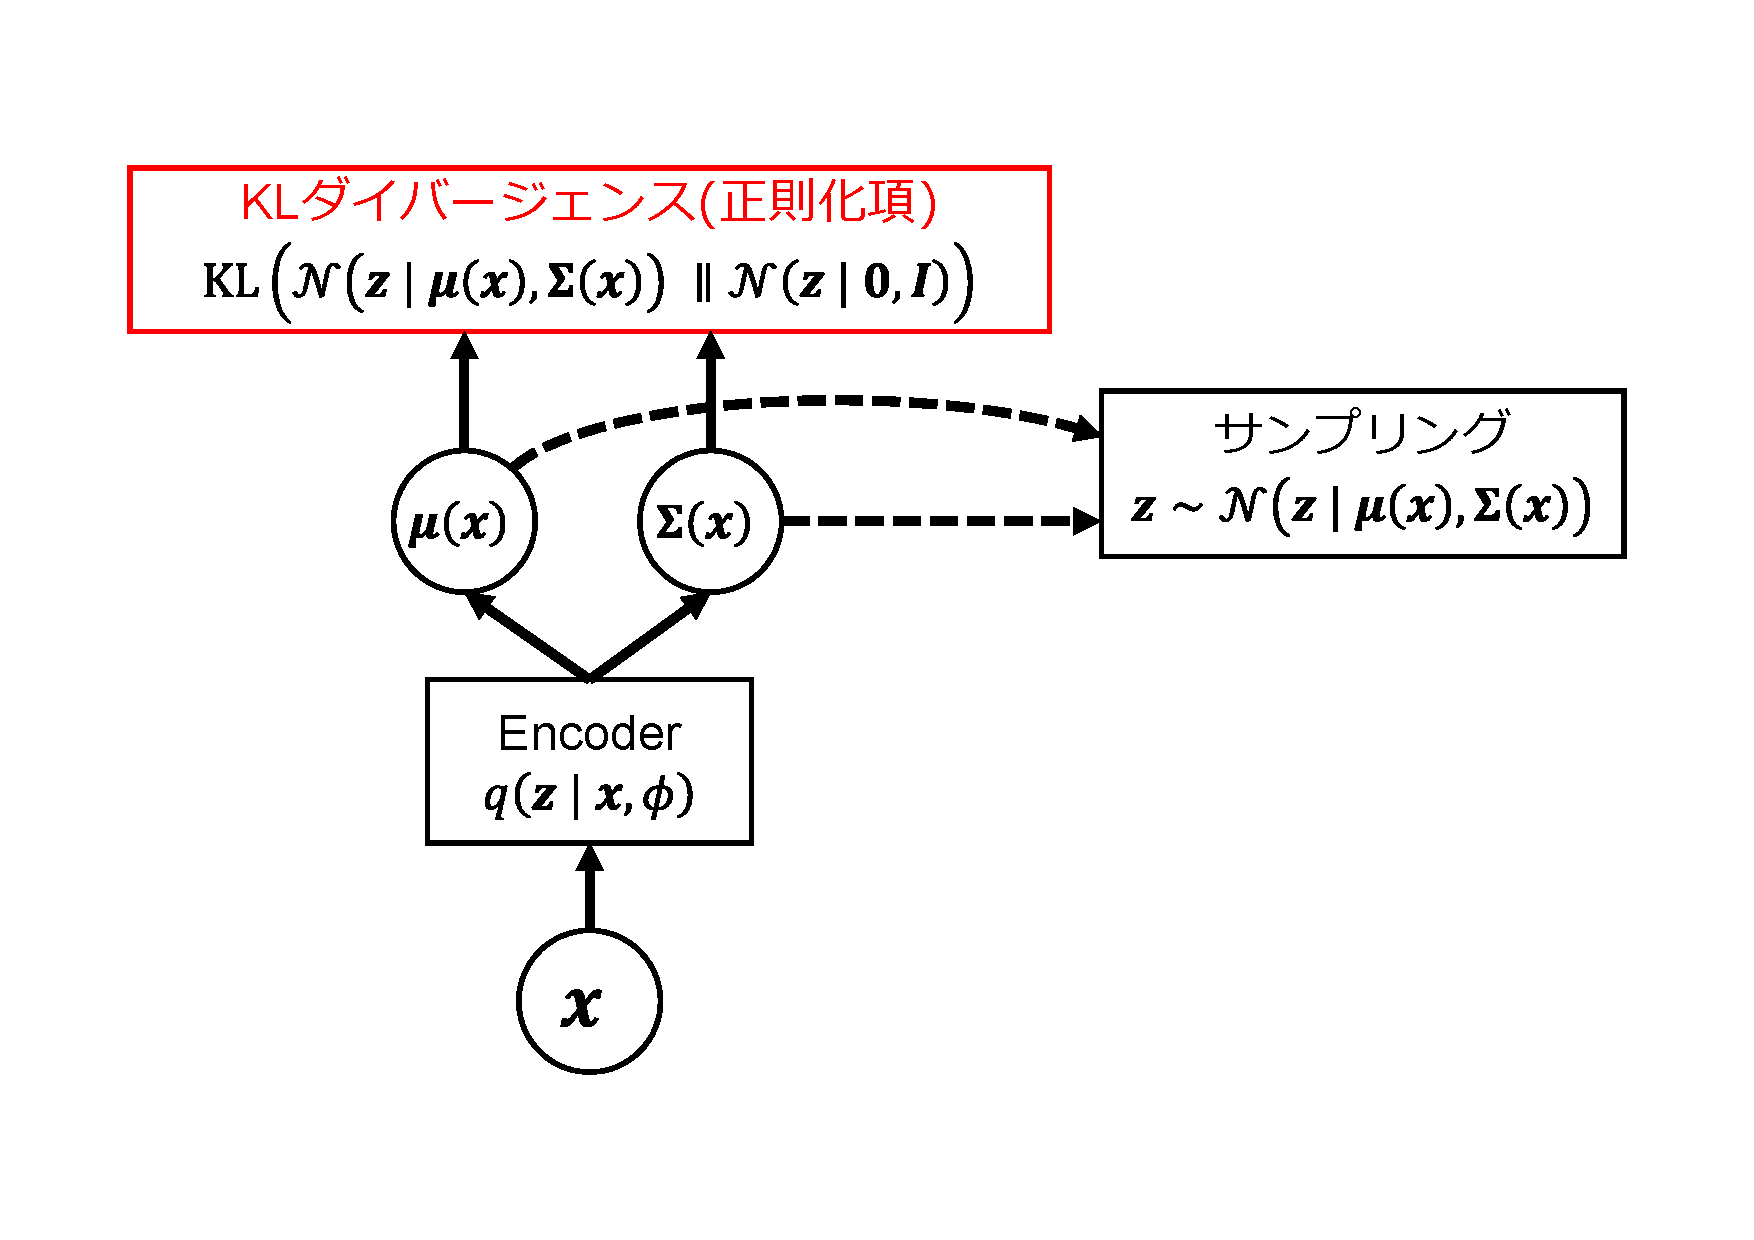
\includegraphics[keepaspectratio,scale=0.3,clip,trim=1cm 1cm 1cm 1cm]{vae-encoder-architecture.pdf}
	\caption{VAEのEncoderの概要}
	\label{fig:vae-encoder-architecture}
\end{figure}

\end{frame}

\begin{frame}{変分自己符号化器(VAE)の理論}
	
\begin{itemize}
	\item Encoderのニューラルネットの構造
	\begin{itemize}
		\item VAEが最初に提案された論文では、隠れ層は1層となっている
		\item 最終層は、$\bm{\mu}_0$と$\sqrt{\bm{\Sigma}_0}$を出力する2つのユニットから成る
		\item $\sqrt{\bm{\Sigma}_0}$とは、行列$\bm{\Sigma}_0$の各要素の平方根を取った行列である
		\newline
		
		\item 隠れ層の重みを$\bm{W}_h$、バイアスを$\bm{b}_h$、活性化関数を$f(\cdot)$、層の出力を$\bm{h}$とする
		\item 隠れ層で行う処理は、次の式で表される
		\begin{equation}
			\bm{h} = f(\bm{W}_h \bm{x} + \bm{b}_h)
		\end{equation}
		
		\item $\bm{\mu}_0$は、重み$\bm{W}_m$とバイアス$\bm{b}_m$を使って、以下のように計算される
		\begin{equation}
			\bm{\mu}_0 = \bm{W}_m \bm{h} + \bm{b}_m
		\end{equation}
		
		\item $\sqrt{\bm{\Sigma}_0}$は、重み$\bm{W}_s$とバイアス$\bm{b}_s$から、以下のように計算される
		\begin{equation}
			\sqrt{\bm{\Sigma}_0} = \bm{W}_s \bm{h} + \bm{b}_s
		\end{equation}
	\end{itemize}
\end{itemize}

\end{frame}

\begin{frame}{変分自己符号化器(VAE)の理論}

\begin{itemize}
	\item Decoderのニューラルネットの入出力
	\begin{itemize}
		\item Decoderは、分布$p(\bm{x} | \bm{z}, \theta)$を表現するニューラルネット
		\item 潜在変数$\bm{z}$から元のデータ$\bm{x}$を復元する
		\newline
	
		\item Decoderの入力は、Encoderによってサンプリングされた$\bm{z}$となる
		\newline
		\item もう少し正確に表現すると、Encoderから出力されるのは、分布のパラメータ$\bm{\mu}, \bm{\Sigma}$である
		\item そして、そのパラメータを使って分布$\mathcal{N}(\bm{z} | \bm{\mu}, \bm{\Sigma})$を構成し、分布から$\bm{z}$をサンプリングする
		\newline
		
		\item Decoderの出力は、復元されたデータ$\bm{y}$である
	\end{itemize}
\end{itemize}

\end{frame}

\begin{frame}{変分自己符号化器(VAE)の理論}

\begin{itemize}
	\item Decoderの損失関数
	\begin{itemize}
		\item 画像データでは通常、各ピクセルの値が$0$から$1$までになるように\alert{スケーリング}されている
		\item このとき、$p(\bm{x} | \bm{z})$は\alert{ベルヌーイ分布}と仮定していることになる
		\newline
		
		\item 出力層のユニット$j$は、$y_j = p(x_j = 1 | \bm{z})$を出力しているとみなせる
		\item $y_j$は、再構成$\bm{y}$の$j$番目の要素であり、元のデータ$\bm{x}$の$j$番目の要素$x_j$と対応する
		\newline
		\item VAEが最初に提案された論文では、隠れ層は1層のみである
		\item 再構成$\bm{y}$は、次のように計算される
		\begin{equation}
			\bm{y} = f_\sigma \left( \bm{W}_o \mathrm{tanh} \left( \bm{W}_h \bm{z} + \bm{b}_h \right) + \bm{b}_o \right)
		\end{equation}
		\item $f_\sigma(\cdot)$は、行列の各要素にシグモイド関数$\sigma(\cdot)$を適用する活性化関数
		\item $\bm{W}_h, \bm{b}_h$は隠れ層の重みとバイアス、$\bm{W}_o, \bm{b}_o$は出力層の重みとバイアス
		\newline
		
		\item このとき$\ln p(\bm{x} | \bm{z})$は次のように記述できる
		\begin{eqnarray}
			\ln p(\bm{x} | \bm{z}) &=& \ln \prod_{j = 1}^D \left( p(x_j = 1 | \bm{z}) \right)^{x_j} \left( p(x_j = 0 | \bm{z}) \right)^{1 - x_j} \nonumber \\
			&=& \ln \prod_j \left( p(x_j = 1 | \bm{z}) \right)^{x_j} \left( 1 - p(x_j = 1 | \bm{z}) \right)^{1 - x_j} \nonumber \\
			&=& \ln \prod_j y_j^{x_j} \left( 1 - y_j \right)^{1 - x_j} \nonumber \\
			&=& \sum_j \left( x_j \ln y_j + \left( 1 - x_j \right) \ln \left( 1 - y_j \right) \right)
		\end{eqnarray}
		
		\item $\bm{z}$は、分布$q(\bm{z} | \bm{x}, \phi)$からサンプリングされている
		\item 従って、上記を最大化することは、$\mathbb{E}_{q(\bm{z})} \left[ \ln p(\bm{x} | \bm{z}) \right]$を最大化することに等しい
		\newline
		
		\item 上記は、$x_j$と$y_j$のいずれもベルヌーイ分布に従う(二値変数)ときの、\alert{負の交差エントロピー}となっていることが分かる
		\item 従って、$\mathbb{E}_{q(\bm{z})} \left[ \ln p(\bm{x} | \bm{z}) \right]$を最大化することは、\alert{交差エントロピーを最小化}することに相当
		\newline
		\item Decoderの損失関数は、以下の\alert{交差エントロピー誤差}として定義できる
		\begin{equation}
			E = - \sum_j \left( x_j \ln y_j + \left( 1 - x_j \right) \ln \left( 1 - y_j \right) \right)
		\end{equation}
		
		\item 元データ$x_j$と、その再構成$y_j$との\alert{差が大きければ大きいほど、上記の誤差は増大}する
		\item これより、上記の誤差は\alert{再構成誤差}(Reconstruction Error)とよばれる
		\newline
		
		\item これより、VAEのEncoderとDecoderは次の図\ref{fig:vae-architecture}のように表せる
	\end{itemize}
\end{itemize}

\end{frame}

\begin{frame}{変分自己符号化器(VAE)の理論}
	
\begin{figure}[h]
	\centering
	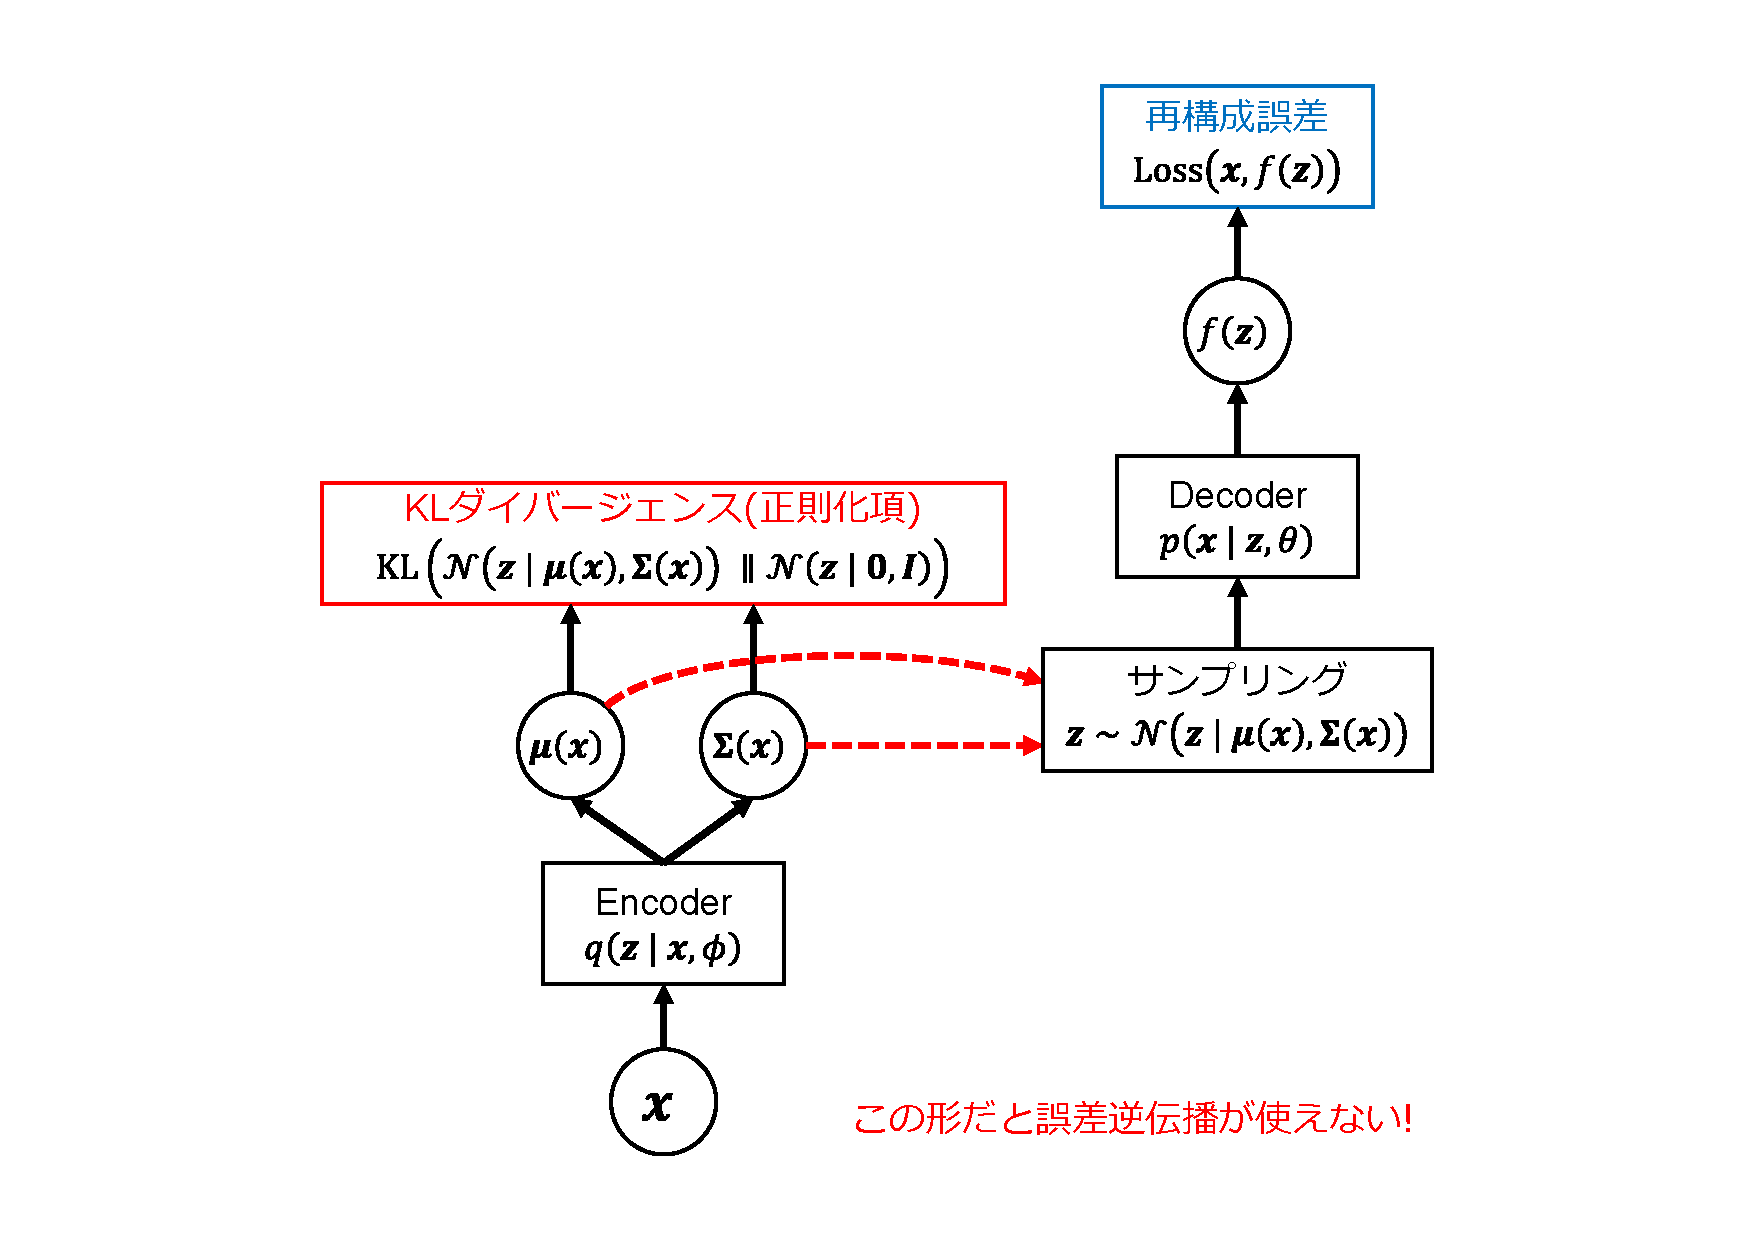
\includegraphics[keepaspectratio,scale=0.3,clip,trim=3cm 1cm 3cm 1cm]{vae-architecture.pdf}
	\caption{VAEのEncoderとDecoderの概要}
	\label{fig:vae-architecture}
\end{figure}

\end{frame}

\begin{frame}{変分自己符号化器(VAE)の理論}

\begin{itemize}
	\item Reparameterization Trick
	\begin{itemize}
		\item VAEが先程の図\ref{fig:vae-architecture}のようであるとき、\alert{大きな問題が生じる}
		\item サンプリングを行うと、計算グラフが途中で途切れるため、\alert{誤差逆伝播法を実行できない}
		\newline
		
		\item そこで、次の図\ref{fig:vae-actual-architecture}のように構成する
		\item $\bm{z} \sim \mathcal{N}(\bm{z} | \bm{\mu}, \bm{\Sigma})$として、$\bm{z}$を分布から直接サンプリングするのではない
		\item $\bm{z}$を、\alert{決定論的な関数}$g(\bm{\epsilon}, \bm{x} | \phi)$から決定する
		\item 但し、$\bm{\epsilon}$は、分布$p(\bm{\epsilon})$からサンプリングされる
		\newline
		
		\item ニューラルネットの最適化には無関係な項$\bm{\epsilon}$と、Encoderのパラメータ$\phi$で$\bm{z}$を表現することで、誤差逆伝播法を実行可能にする
		\item このテクニックを、\alert{Reparameterization Trick}という
		\newline
		
		\item $\bm{\epsilon} \sim \mathcal(\bm{\epsilon} | \bm{0}, \bm{I})$とすれば、$\bm{z}$は次のように計算できる
		\begin{equation}
			\bm{z} = g(\bm{\epsilon}, \bm{x} | \phi) = \bm{\mu} + \bm{\Sigma}^\frac{1}{2} \bm{\epsilon}
		\end{equation}
		
		\item 共分散行列$\bm{\Sigma}$が対角行列であれば、上記の$\bm{\Sigma}^\frac{1}{2} \bm{\epsilon}$は、単なる要素ごとの積(対角行列の各要素を並べたベクトルと、$\bm{\epsilon}$の要素ごとの積)として書ける
		\newline
		
		\item $\bm{z}$の式は以下のように導出できる
		\newline
		
		\item 確率変数$\bm{z}, \bm{\epsilon}$間の関係が、次のようになっているとする
		\begin{equation}
			\bm{z} = \bm{\mu} + \bm{U} \bm{\Lambda}^\frac{1}{2} \bm{\epsilon}
		\end{equation}
		
		\item 但し、正定値対称行列$\bm{\Sigma}$が、固有値分解によって$\bm{\Sigma} = \bm{U} \bm{\Lambda} \bm{U}^T = \bm{U} \bm{\Lambda}^\frac{1}{2} \left( \bm{U} \bm{\Lambda} \right)^T$と表せるとする
		\item $\bm{U}$は固有ベクトルを並べた行列、$\bm{\Lambda}$は対角成分に固有値をもつ対角行列とする
		\newline
		
		\item 確率分布$p(\bm{z})$と$p(\bm{\epsilon})$との関係は、ヤコビ行列$\bm{J} = \partial \bm{\epsilon} / \partial \bm{z}$により次のように記述できる
		\begin{equation}
			p(\bm{z}) = p(\bm{\epsilon}) | \det \left( \bm{J} \right) | = p(\bm{\epsilon}) \left| \det \left( \frac{\partial \bm{z}}{\partial \bm{\epsilon}} \right) \right|
		\end{equation}
		
		\item ヤコビ行列$\bm{J}$を計算すると次のようになる
		\begin{equation}
			\bm{J} = \frac{\partial \bm{\epsilon}}{\partial \bm{z}} = \frac{\partial}{\partial \bm{z}} \left( \left( \bm{U} \bm{\Lambda}^\frac{1}{2} \right)^{-1} \left( \bm{z} - \bm{\mu} \right) \right) = \left( \left( \bm{U} \bm{\Lambda}^\frac{1}{2} \right)^{-1} \right)^T
		\end{equation}
		
		\item ヤコビ行列$\bm{J}$の行列式は次のようになる
		\begin{eqnarray}
			\det \left( \bm{J} \right) &=& \left| \left( \left( \bm{U} \bm{\Lambda}^\frac{1}{2} \right)^{-1} \right)^T \right| \nonumber \\
			&=& \left| \left( \bm{U} \bm{\Lambda}^\frac{1}{2} \right)^{-1} \right| \qquad (\because |\bm{A}^T| = |\bm{A}|) \nonumber \\
			&=& \frac{1}{\left| \bm{U} \bm{\Lambda}^\frac{1}{2} \right|} \qquad \left( \because |\bm{A}^{-1}| = \frac{1}{|\bm{A}|} \right) \nonumber \\
		\end{eqnarray}
		
		\item $\bm{\Sigma}$の行列式は次のように表せる
		\begin{equation}
			| \bm{\Sigma} | = \left| \bm{U} \bm{\Lambda}^\frac{1}{2} \left( \bm{U} \bm{\Lambda}^\frac{1}{2} \right)^T \right| = \left| \bm{U} \bm{\Lambda}^\frac{1}{2} \right| \left| \left( \bm{U} \bm{\Lambda}^\frac{1}{2} \right)^T \right| = \left| \bm{U} \bm{\Lambda}^\frac{1}{2} \right|^2
		\end{equation}
		
		\item 従って$\left| \bm{U} \bm{\Lambda}^\frac{1}{2} \right| = \left| \bm{\Sigma} \right|^\frac{1}{2}$である
		\item $\bm{\Sigma}$は正定値である($\left| \bm{\Sigma} \right| > 0$)から、$\left| \bm{\Sigma} \right|^\frac{1}{2} = \left| \bm{U} \bm{\Lambda}^\frac{1}{2} \right| > 0$が成立し、$\bm{U} \bm{\Lambda}^\frac{1}{2}$も正定値行列となる
		\item これより、逆行列$\left( \bm{U} \bm{\Lambda}^\frac{1}{2} \right)^{-1}$が存在するので、ヤコビ行列$\bm{J}$は計算できることが確認される
		\newline
		\item ヤコビ行列$\bm{J}$の行列式の絶対値は、次のようになる
		\begin{equation}
			\left| \det(\bm{J}) \right| = \left| \frac{1}{\left| \bm{U} \bm{\Lambda}^\frac{1}{2} \right|} \right| = \left| \frac{1}{\left| \bm{\Sigma} \right|^\frac{1}{2}} \right| = \frac{1}{\left| \bm{\Sigma} \right|^\frac{1}{2}}
		\end{equation}
		
		\item $p(\bm{\epsilon})$がガウス分布$\mathcal{N}(\bm{\epsilon} | \bm{0}, \bm{I})$であるとすると、$p(\bm{z})$は次のようになる
		\begin{eqnarray}
			p(\bm{z}) &=& p(\bm{\epsilon}) \left| \det \left( \frac{\partial \bm{z}}{\partial \bm{\epsilon}} \right) \right| \nonumber \\
			&=& \frac{1}{(2\pi)^\frac{K}{2}} \exp \left( -\frac{1}{2} \bm{\epsilon}^T \bm{\epsilon} \right) \frac{1}{|\bm{\Sigma}|^\frac{1}{2}}
		\end{eqnarray}
		
		\item ここで、指数関数の中身は次のように書ける
		\begin{eqnarray}
			&& \left( \bm{z} - \bm{\mu} \right)^T \bm{\Sigma}^{-1} \left( \bm{z} - \bm{\mu} \right) \nonumber \\
			&=& \left( \bm{U} \bm{\Lambda}^\frac{1}{2} \bm{\epsilon} \right)^T \left( \bm{U} \bm{\Lambda} \bm{U}^T \right)^{-1} \left( \bm{U} \bm{\Lambda}^\frac{1}{2} \bm{\epsilon} \right) \nonumber \\
			&=& \bm{\epsilon}^T \left( \bm{\Lambda}^\frac{1}{2} \right)^T \bm{U}^T \left( \bm{U}^T \right)^{-1} \bm{\Lambda}^{-1} \bm{U}^{-1} \bm{U} \bm{\Lambda}^\frac{1}{2} \bm{\epsilon} \nonumber \\
			&=& \bm{\epsilon}^T \left( \bm{\Lambda}^\frac{1}{2} \right)^T \bm{\Lambda}^{-1} \bm{\Lambda}^\frac{1}{2} \bm{\epsilon} \nonumber \\
			&=& \bm{\epsilon}^T \bm{\Lambda}^\frac{1}{2} \bm{\Lambda}^{-1} \bm{\Lambda}^\frac{1}{2} \bm{\epsilon} \nonumber \\
			&=& \bm{\epsilon}^T \bm{\epsilon}
		\end{eqnarray}
		
		\item これより、$p(\bm{z})$は平均$\bm{\mu}$、共分散行列$\bm{\Sigma}$のガウス分布である
		\begin{eqnarray}
			p(\bm{z}) &=& \frac{1}{(2\pi)^\frac{K}{2}} \exp \left( -\frac{1}{2} \bm{\epsilon}^T \bm{\epsilon} \right) \frac{1}{|\bm{\Sigma}|^\frac{1}{2}} \nonumber \\
			&=& \frac{1}{(2\pi)^\frac{K}{2}} \frac{1}{|\bm{\Sigma}|^\frac{1}{2}} \exp \left( -\frac{1}{2} \left( \bm{z} - \bm{\mu} \right)^T \bm{\Sigma}^{-1} \left( \bm{z} - \bm{\mu} \right) \right) \\
			&=& \mathcal{N}(\bm{z} | \bm{\mu}, \bm{\Sigma})
		\end{eqnarray}
		
		\item $\bm{z} \sim \mathcal{N}(\bm{z} | \bm{\mu}, \bm{\Sigma})$について、共分散行列$\bm{\Sigma}$が既に対角行列であれば、$\bm{U} = \bm{I}$、$\bm{\Lambda} = \bm{\Sigma}$であるので、結局以下が言える
		\begin{equation}
			\bm{z} = \bm{\mu} + \bm{U} \bm{\Lambda}^\frac{1}{2} \bm{\epsilon} = \bm{\mu} + \bm{\Sigma}^\frac{1}{2} \bm{\epsilon}
		\end{equation}
	\end{itemize}
\end{itemize}

\end{frame}

\begin{frame}{変分自己符号化器(VAE)の理論}
	
\begin{figure}[h]
	\centering
	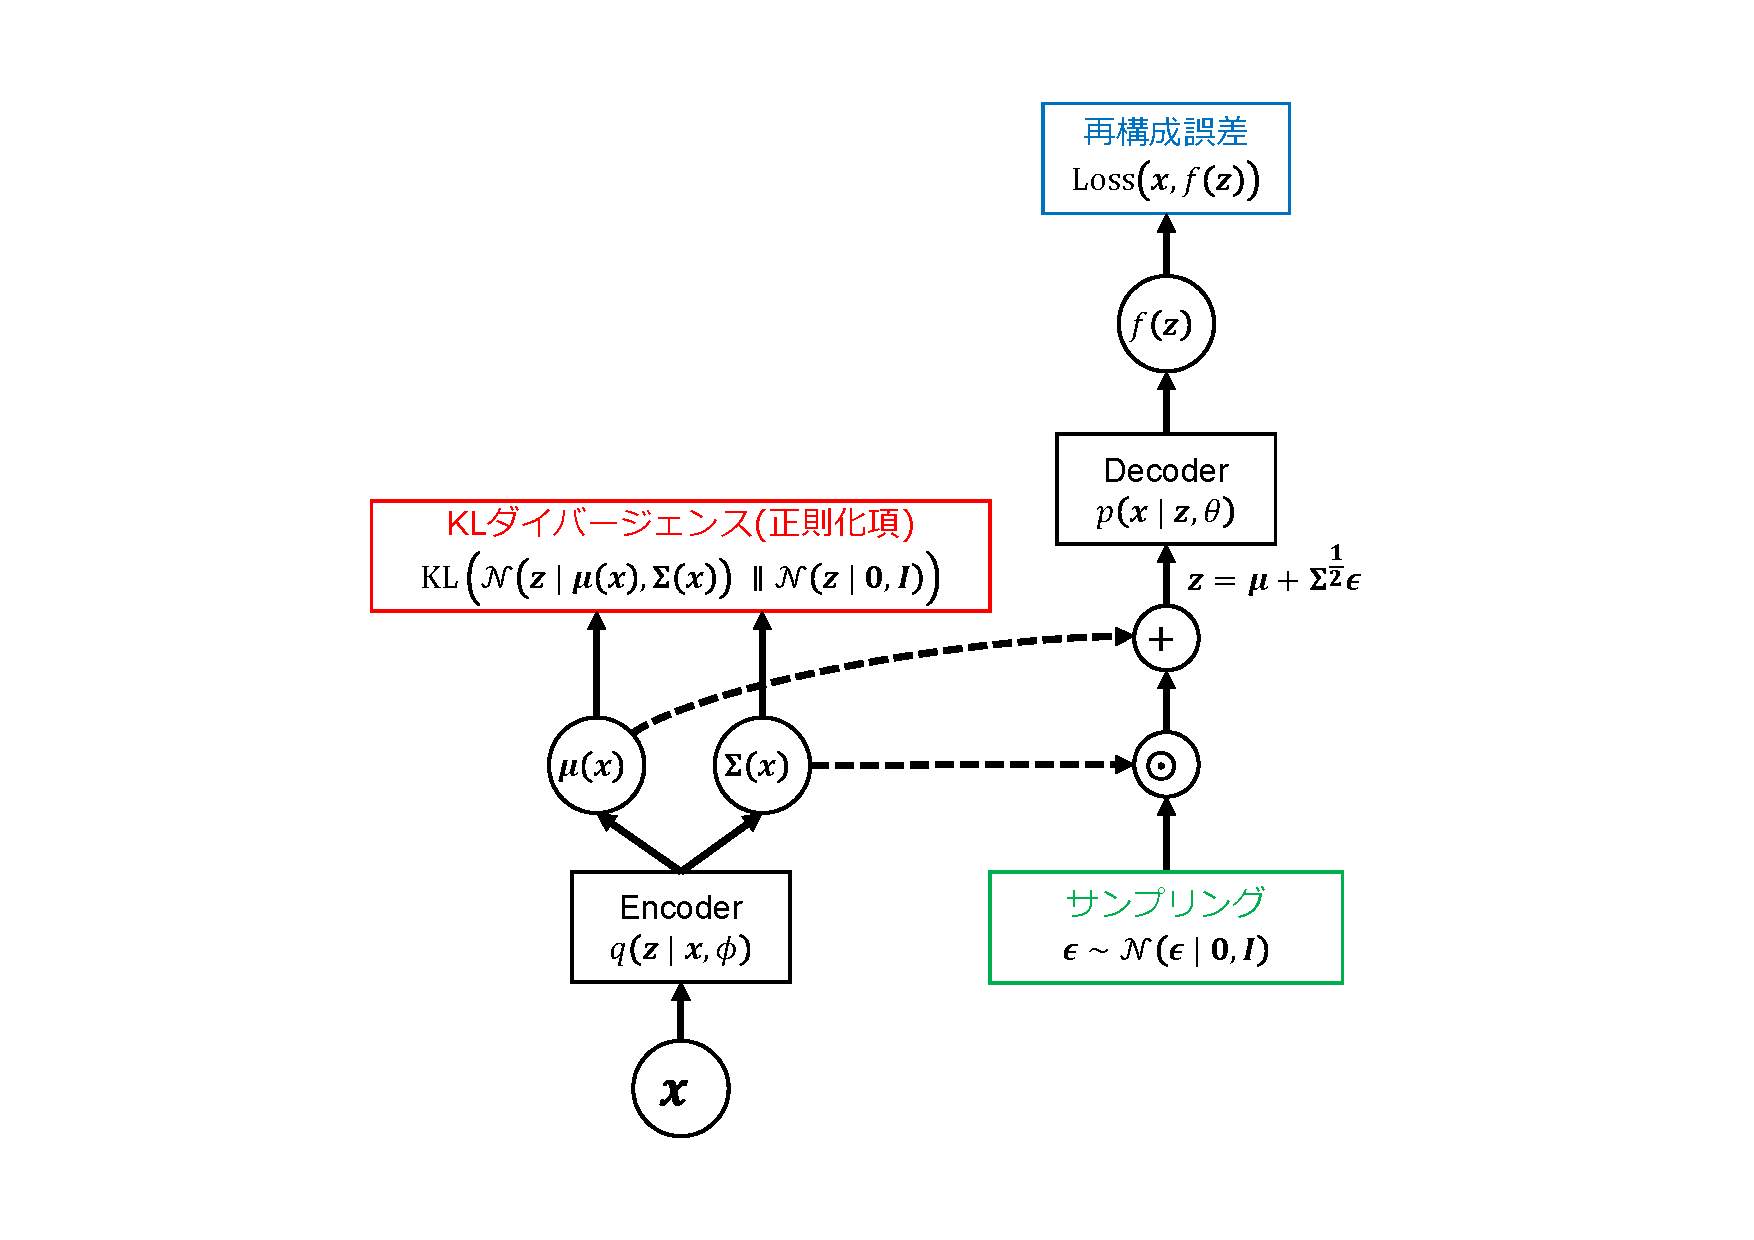
\includegraphics[keepaspectratio,scale=0.3,clip,trim=3cm 1cm 3cm 1cm]{vae-actual-architecture.pdf}
	\caption{VAEの構造}
	\label{fig:vae-actual-architecture}
\end{figure}

\end{frame}

\end{document}
